\documentclass{article}
\usepackage{amsmath,amssymb}
\usepackage{latexsym}
\usepackage{graphicx}
\usepackage{verbatim}
\usepackage[framed,numbered,autolinebreaks,useliterate]{mcode}
\usepackage{fancyhdr}
\pagestyle{fancy}

\title{Numerical Analysis Assignment \#1}
\author{Xinglu Wang}
\renewcommand{\baselinestretch}{1}
\newcommand\abs[1]{\left\lvert #1 \right\rvert}
\setlength{\textwidth}{16cm}
\setlength{\textheight}{23cm}
\setlength{\oddsidemargin}{0.5pc}
\setlength{\evensidemargin}{-3.5pc}
\setlength{\topmargin}{-4.5pc}
\setlength{\columnsep}{1.5pc}
\makeatletter
\def\@seccntformat#1{%
  \expandafter\ifx\csname c@#1\endcsname\c@section\else
  \csname the#1\endcsname\quad
  \fi}
\makeatother

%\fancyhf{}
\fancyheadoffset{1.5pc}
\lhead{Numerical Analysis Assignment \#1 \qquad Xinglu Wang \quad 3140102282}
%\chead{  Xinglu Wang \quad 3140102282}
\rhead{ \thepage}
%\cfoot{center of the footer!}
\renewcommand{\headrulewidth}{0.2pt}
%\renewcommand{\footrulewidth}{0.4pt}


\begin{document}

\begin{center}
{ \Large \bf Numerical Analysis Assignment \#1}
\vskip1.0cm
Xinglu Wang \qquad Student Number: 3140102282\\
College of Information Science \& Electronic Engineering, Zhejiang University
\end{center}
\vskip1.0cm
It is my first time to write an article with \LaTeX{} and in English. I am quite exciting and find myself learned a lot in this wonderful course! \\
After programming and debugging, I am impressed that Fix-Point method is hard to find a good $g(x)$, and when I choose $g(x)=x-\frac{f(x)}{{f'}(x)}$ , this method will be sensitive to initial value.
\section{Problem 1:}
\paragraph{a.}
This problem satisfies condition of Intermediate Value Theorem, since  $ f\in C[a,b]$ \\
Meanwhile,
$$ \min (f({x_1}),f({x_2})) \le \frac{{f({x_1}) + f({x_2})}}{2} \le \max (f({x_1}),f({x_2}))$$
Therefore,
\[\exists \xi  \in [{x_1},{x_2}]:\qquad f(\xi ) = \frac{{f({x_1}) + f({x_2})}}{2}\]

\paragraph{b.}
Similarly, because $c_1$ and $c_2$ is positive, $f(\xi )$ the weighted average of $f(x_1)$ and $f(x_2)$, \\
which means,
\[\min (f({x_1}),f({x_2})) \le \frac{{{c_1}f({x_1}) + {c_2}f({x_2})}}{{{c_1} + {c_2}}} \le \max (f({x_1}),f({x_2}))\]
Therefore,
\[\exists \xi  \in [{x_1},{x_2}]:\qquad f(\xi ) = \frac{{{c_1}f({x_1}) + {c_2}f({x_2})}}{{{c_1} + {c_2}}}\]
\paragraph{c.}
When $f(x)=x, \quad
\left\{ {\begin{array}{*{20}{c}}
{{c_1} =  - 1}\\
{{c_2} = 2}
\end{array}} \right. and \quad
\left\{ {\begin{array}{*{20}{c}}
{{x_1} = 1}\\
{{x_2} = 2}
\end{array}} \right. ,
$
\[\frac{{{c_1}f({x_1}) + {c_2}f({x_2})}}{{{c_1} + {c_2}}} = 2 \notin [1,2]\]
In this condition, therefore
\[!\exists \xi  \in [1,2]:\qquad f(\xi ) = \frac{{{c_1}f({x_1}) + {c_2}f({x_2})}}{{{c_1} + {c_2}}}\]

\section{Problem 2:}
\begin{description}
\item\textbf{a.}\\
This problem satisfies Mean Value Theorem, since $f \in C[a,b]$ and f is differentiable on $(a,b)$,  therefore the absolute error is
\[\left| {\tilde f({x_0}) - f({x_0})} \right| = \left| {f'(\xi )} \right|\left| \varepsilon  \right| \approx \varepsilon \left| {f'({x_0})} \right|  \text{  ,where  } x_0-\varepsilon \leq \xi \leq x_0+\varepsilon \]
And the relative error is
\[\left| {\frac{{\tilde f({x_0}) - f({x_0})}}{{f({x_o})}}} \right| = \left| {f'(\xi )} \right|\left| {\frac{\varepsilon }{{f({x_0})}}} \right| \approx \varepsilon \frac{{\left| {f'({x_0})} \right|}}{{\left| {f({x_0})} \right|}} \text{  , where  } x_0-\varepsilon \leq \xi \leq x_0+\varepsilon \]
\item\textbf{b.}
   \begin{description}
         \item[i] Submit $\varepsilon $ and $x_0 $ into formula above, we know the absolute error is
             $1.3591\times {{10}^{-5}}$ and the relative is
 $5.0000\times {{10}^{-6}}$
         \item[ii] Similarly, the absolute error is
 $2.7015\times {{10}^{-6}}$.
and the relative is
$3.2105\times {{10}^{-6}}$.
       \end{description}
\item\textbf{c.}
\begin{description}
\item[i]
Bound of absolute error is $1.1013$  and the relative is $5.0000\times {{10}^{-5}}$.
\item[ii]
Bound of absolute error is $4.1954\times {{10}^{-5}}$  and the relative is $7.7118\times {{10}^{-5}}$.
\end{description}

\end{description}
We find that \textbf{\emph{(ii)}} in \textbf{c} is quite special, which shows that for $e^{x}$ relative error is more than absolute one because of its rapid exponential incasement!

\section{Problem 3:}
    \paragraph {a:}
    \textbf{\emph{(i)}} \[A=\frac{4}{5}+\frac{1}{3}=\frac{17}{15}\]
    \textbf{\emph{(ii)}} \[A=chop(chop(\frac{4}{5})+chop(\frac{1}{3}))=chop(0.800+0.333)=1.133\]
     \textbf{\emph{(iii)}} \[A=round(0.800+0.333)=1.133\]
    \textbf{\emph{(iv)}} Relative error is $0.029\%$ and $0.029\%$

    \paragraph{b:}
    \textbf{\emph{(i)}} \[A=\frac{20}{33}-\frac{3}{20}=\frac{301}{660}\]
    \textbf{\emph{(ii)}}
    \[A=chop(chop(0.605)-chop(\frac{3}{20}))=chop(0.605-0.150)=0.455\]
   \textbf{\emph{(iii)}} \[A=round(0.606-0.150)=0.456\]
    \textbf{\emph{(iv)}} Relative error is $0.2331\%$ and $0.0133\%$

\section{Problem 4:}
\paragraph{a.}When $\gamma < \beta$ and $\gamma <\alpha$
\[\mathop{\lim }_{x\to 0}\frac{F(x)-{{c}_{1}}{{L}_{1}}-{{c}_{2}}{{L}_{2}}}{{{x}^{\gamma }}}=\mathop{\lim }_{x\to 0}\frac{{{c}_{1}}O({{x}^{\alpha }})+{{c}_{2}}O({{x}^{\beta }})}{{{x}^{\gamma }}}=0\]
which is equal to \[F(x)={{c}_{1}}{{L}_{1}}+{{c}_{2}}{{L}_{2}}+O({{x}^{\gamma }})\]
\paragraph{b.}When $\gamma < \beta$ and $\gamma <\alpha$
\[\mathop{\lim }_{x\to 0}\frac{G(x)-{{L}_{1}}-{{L}_{2}}}{{{x}^{\gamma }}}=\mathop{\lim }_{x\to 0}\frac{O({{({{c}_{1}}x)}^{\alpha }})+O({{({{c}_{2}}x)}^{\beta }})}{{{x}^{\gamma }}}=0\]
\section{Problem 5:}
Implement the Bisection method in C or matlab and find solutions accurate to within  for the following problems. (List the midpoints in each iteration as well) .
\paragraph{a.}	${{e}^{x}}-{{x}^{2}}+3x-2=0 \text{ \quad for } 0\le x\le 1$
\\After applying  the Bisection method , the value of x is 0.257530212402344, the midpoint is listed and ploted below:
\begin{center}
\begin{tabular}{ |l|r| }
  \hline
  \multicolumn{2}{|c|}{Midpoint List} \\
  \hline
0.5 & 0.256836 \\
0.25 & 0.257324 \\
0.375 & 0.257568 \\
0.3125 & 0.257446 \\
0.28125 & 0.257507 \\
0.265625 & 0.257538 \\
0.257813 & 0.257523 \\
0.253906 & \multicolumn{1}{r|}{ 0.257530  } \\ \cline{2-2}
0.255859 \\ \cline{1-1}
\end{tabular}
\end{center}

\begin{center}
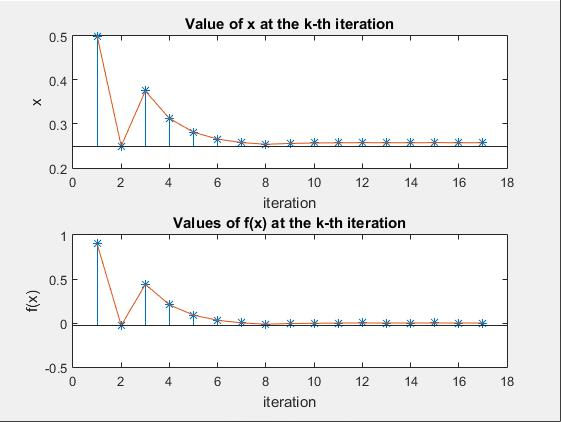
\includegraphics[height=8.5 cm]{fig5_a.jpg} \\
Fig.5.1 Plot iteration points for Bisection Method
\end{center}

\paragraph{b.}	$x\cos x-2{{x}^{2}}+3x-1=0  \text{ \quad for } 0.2\le x\le 0.3 \text{ and } 1.2\le x\le 1.3$
\\ The root of $x\cos x-2{{x}^{2}}+3x-1=0$  with the initial condition of $0.2\le x\le 0.3$ is 0.297528076171875, the midpoint is listed and ploted below:
\begin{center}
\begin{tabular}{ |l|r| }
  \hline
  \multicolumn{2}{|c|}{Midpoint List} \\
  \hline
0.25& 0.297266 \\
0.275& 0.297461 \\
0.2875& 0.297559 \\
0.29375& 0.297510 \\
0.296875& 0.297534 \\
0.298438& 0.297522 \\
0.297656& 0.297528 \\
  \hline
\end{tabular}
\end{center}
\begin{center}
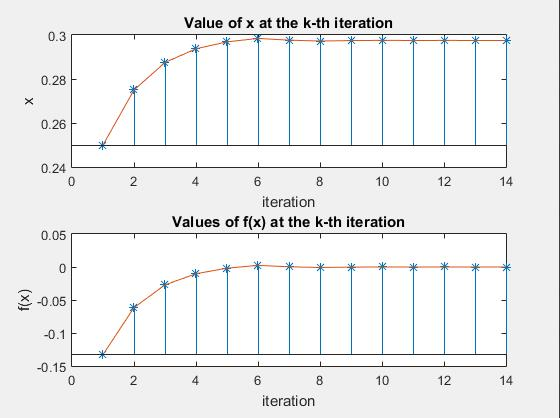
\includegraphics[height=8.5 cm]{fig5_b1.jpg} \\
Fig.5.a.1 Plot iteration points for Bisection Method
\end{center}

The root of $x\cos x-2{{x}^{2}}+3x-1=0$  with the initial condition of $1.2\le x\le 1.3$ is 1.256622314453125, the midpoint is listed and ploted below:
\begin{center}
\begin{tabular}{ |l|r| }
  \hline
  \multicolumn{2}{|c|}{Midpoint List} \\
  \hline
1.25 & 1.25664 \\
1.275 & 1.25645 \\
1.2625 & 1.25654 \\
1.25625 & 1.25659 \\
1.25937 & 1.25662 \\
1.25781 & 1.25663 \\
1.25703 & 1.25662 \\
  \hline
\end{tabular}
\end{center}
\begin{center}
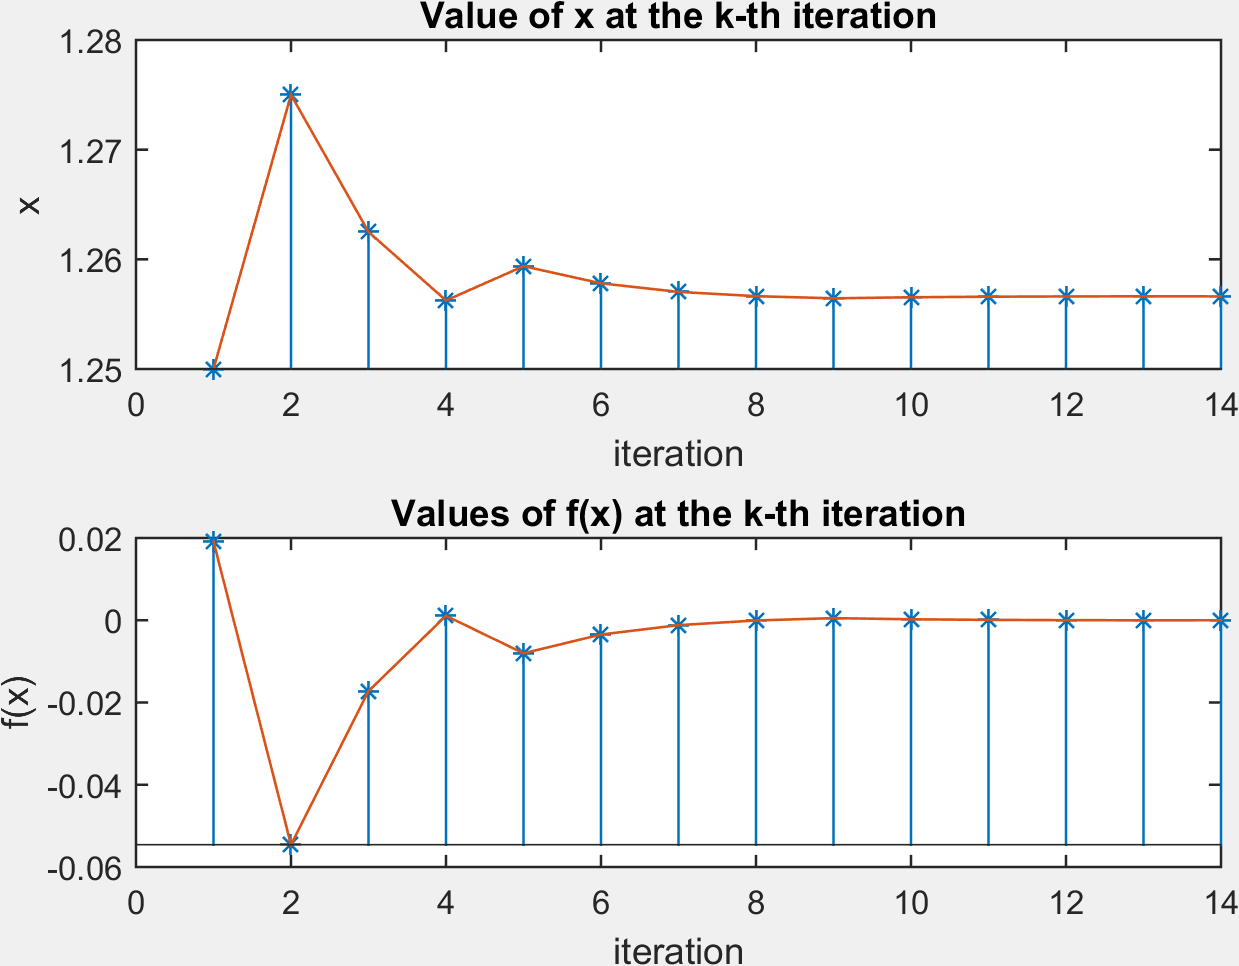
\includegraphics[height=8.5 cm]{fig5_b2.png} \\
Fig.5.a.2 Plot iteration points for Bisection Method
\end{center}
Usage of Bisection Method and process to solve problem is shown below:

\begin{lstlisting}
func1=@(x) exp(x)-x^2+3*x-2; %for problem a
func2=@(x) x*cos(x)-2*x^2+3*x-1; %for problem b
res1=Bisection(func1,[0,1],10^-5,1000)
%specify function_handle,left and right initial valuer,TOL and max iteration times correspondingly
res2=Bisection(func2,[0.2,0.3],10^-5,1000)
res3=Bisection(func2,[1.2,1.3],10^-5,1000)
\end{lstlisting}
The implement of Bisection Method is shown below:
\lstinputlisting{Bisection.m}


\section{Problem 6:}
{\bf{\emph{PROBLEM:}}}
Implement the fixed-point iteration method in C or matlab and find solutions accurate to within ${{10}^{-2}}$ for the following problems. (List pn in each iteration as well).
\paragraph{a.}	$2\sin \pi x+x=0$ on [1, 2], use ${{p}_{0}}=1$
\\{\bf{\emph{SOLUTION}}}
For this problem we should be careful the initial guess result from Bisection method, A crude estimate reduce to divergence while an accurate one make Fix-Point method not function.
\begin{itemize}
  \item Estimate the initial value by plot or Monte Carlo method.
  Then we can use Bisection method to reduce TOL to suitable value. Here I just estimate the x coordination of intersection point.
  \item Then we construct a suitable $g(x)=x$ from $f(x)=0$, and my choice is $g(x)=x-\frac{f(x)}{{f}'(x)}$, which is exactly another form of Newton method. Apparently, Newton method is a kind of Fix-Point method, with a perfect $g(x)$ satisfies $\left| {f}'(p) \right|<1$ automatically. I love this merit.
  \item Now that the g(x) we choose has satisfies $\left| {f}'(p) \right|<1$ automatically, as Fix-Point method show, we just need to generate x via g(x) step by step.
\end{itemize}
For problem a, the initial step for estimation is shown below, which contain $f_1(x)=x$ and $f_2(x)=-2sin(\pi x)$. Apparently, to choose $g(x)=-2sin(\pi x)$ is not proper.
\begin{center}
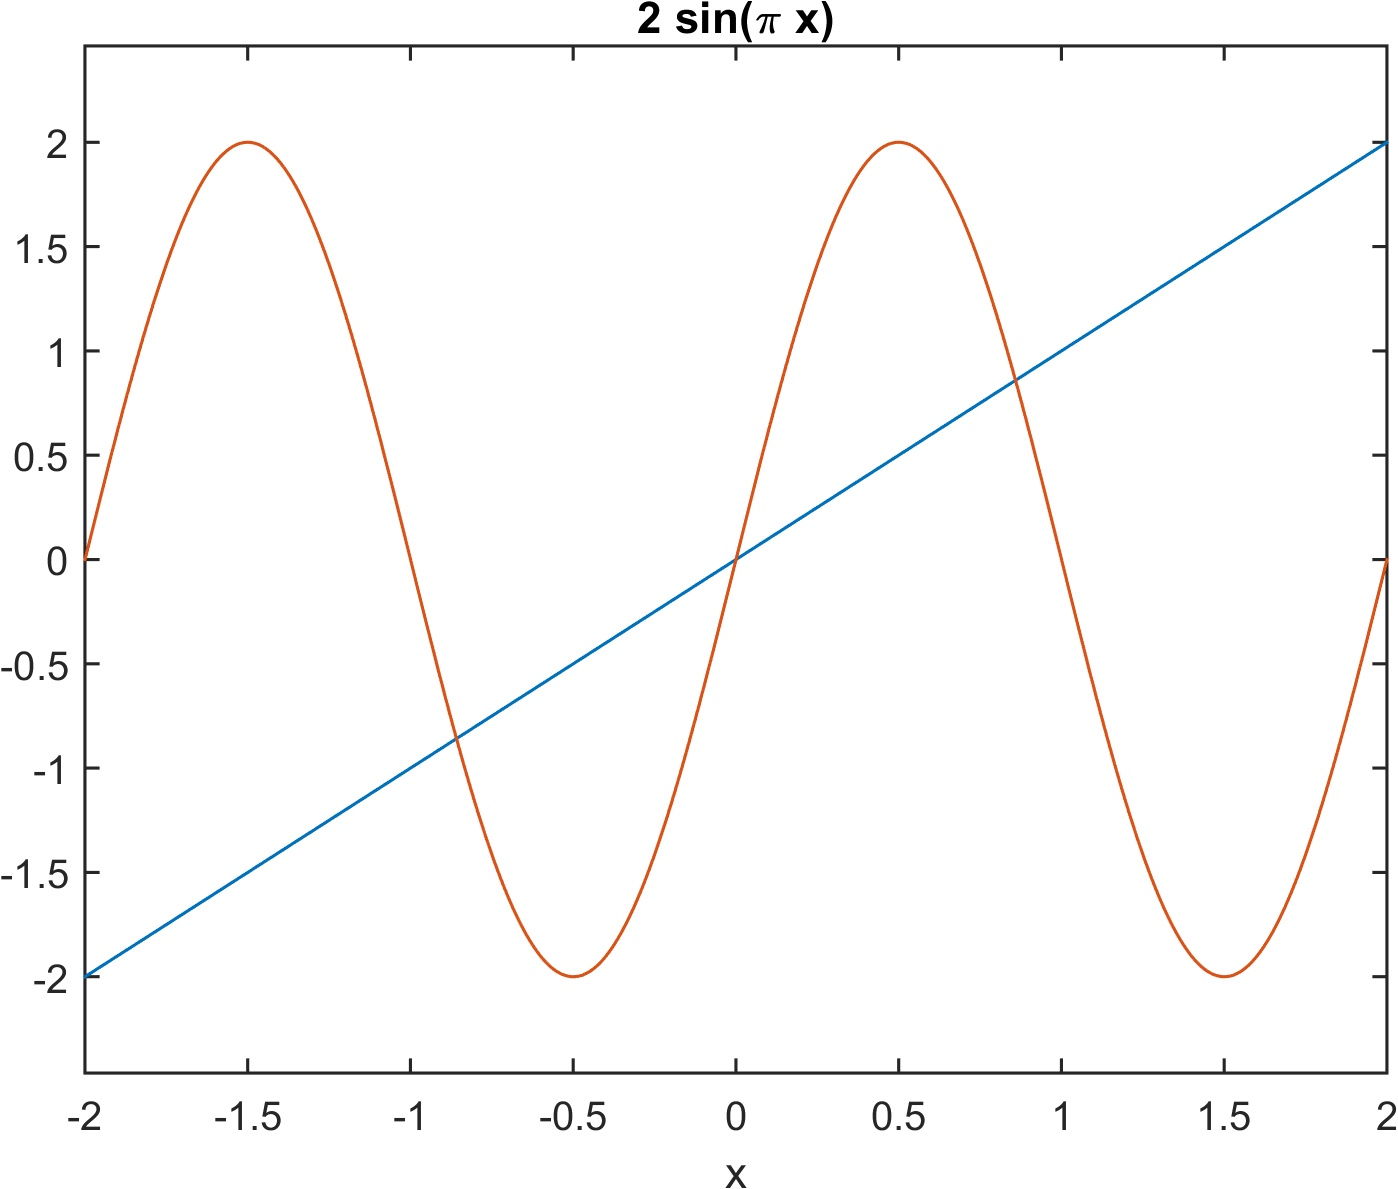
\includegraphics[height=6.5 cm]{sin.jpg} \\
Fig.5.a.1 Figure for estimation.
\end{center}
My first mistake is shown below, because choose $g(x)=x-\frac{{f}'(x)}{f(x)}$ instead of $g(x)=x-\frac{f(x)}{{f}'(x)}$ , the root divergent! I think I will never forget this formula, and I am impressed that computer will be correct if I choose a correct algorithm.
\begin{center}
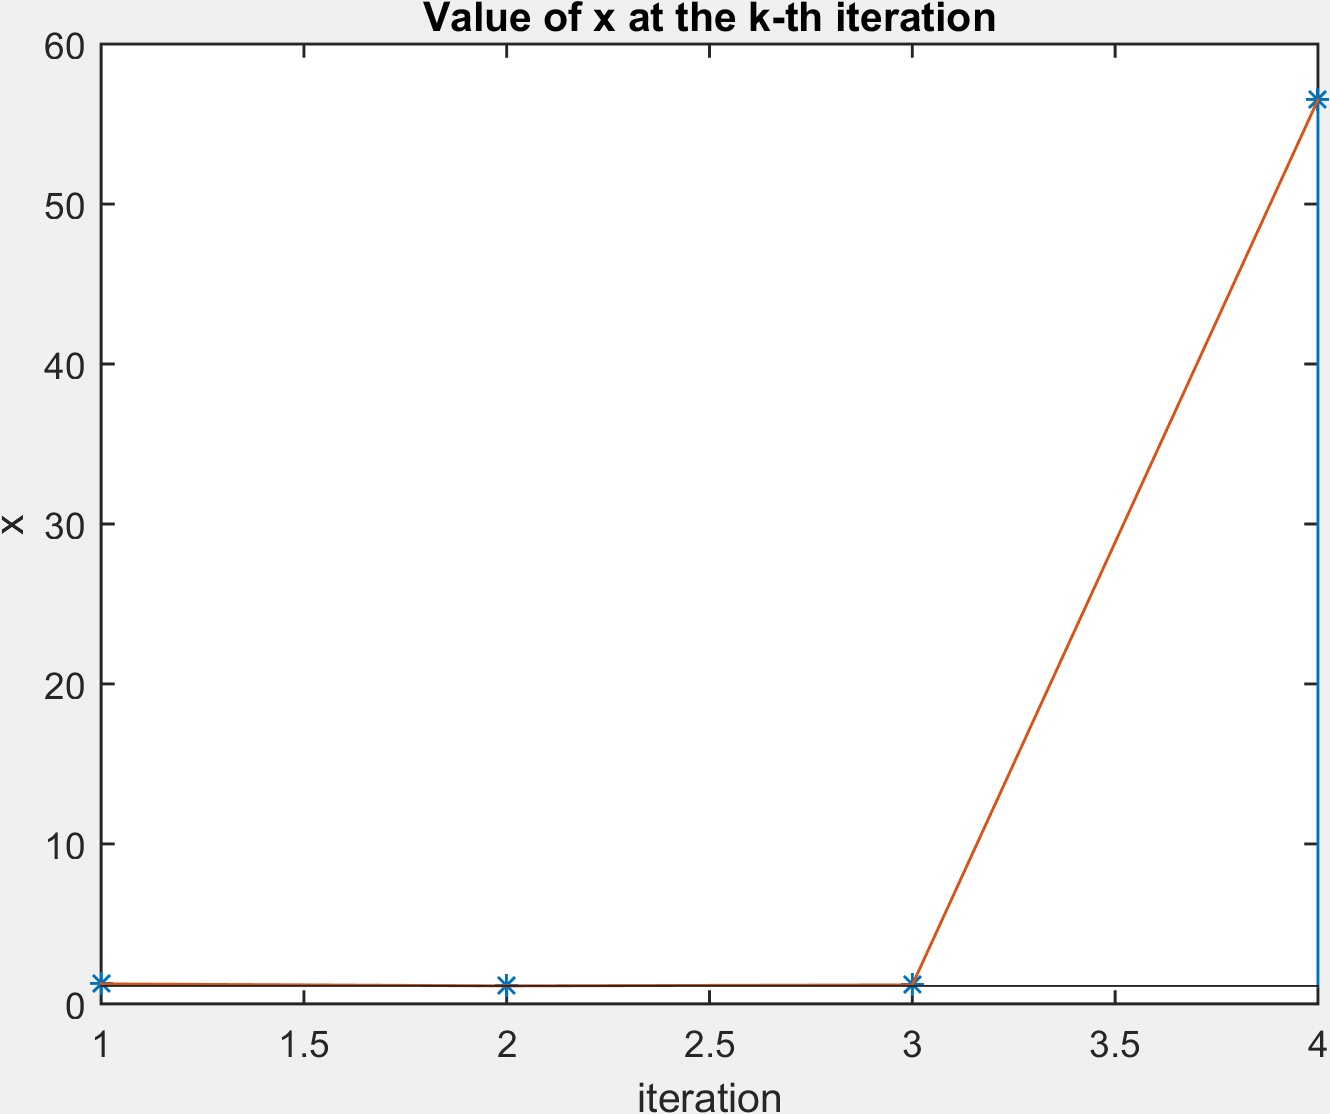
\includegraphics[height=6.5 cm]{divergence.jpg} \\
Fig.5.a.2 the result of my first time mistake.
\end{center}

The root for $2\sin \pi x+x=0$ on [1, 2], use ${{p}_{0}}=1$ is 1.206034907345460, for the initial point is 1 which excludes the root near 1.6.
Iterations points and graph are shown below
\begin{center}
\begin{tabular}{ |l| }
\hline
 1.000000000000000\\
   1.189279751107925\\
   1.205656458413502\\
   1.206034907345460\\

\hline
\end{tabular}
\end{center}

\begin{center}
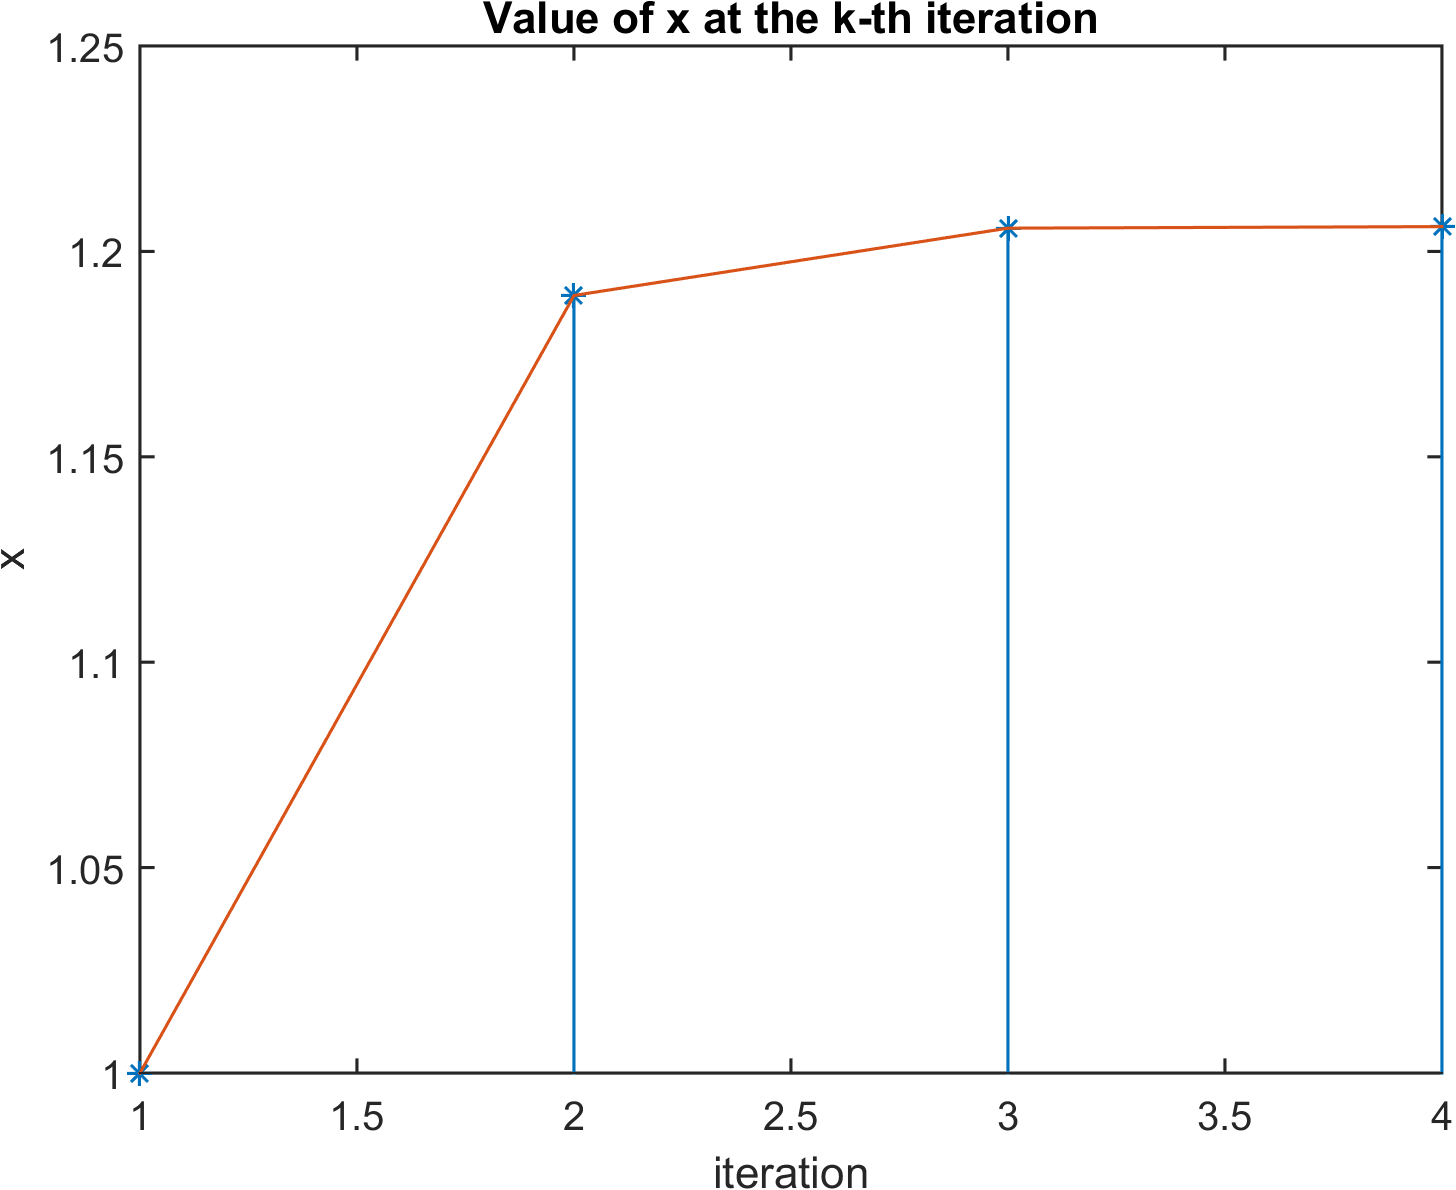
\includegraphics[height=7.5 cm]{fig6(1).png} \\
Fig.5.a.3 Plot iteration points for Bisection Method
\end{center}

\paragraph{b.}	$3{{x}^{2}}-{{e}^{x}}=0$
\\First we must plot the function to estimate.There are three roots. After running programme, we find they are  -0.458962274194841, 0.910017665783406 and 3.733079065494898.
\begin{center}
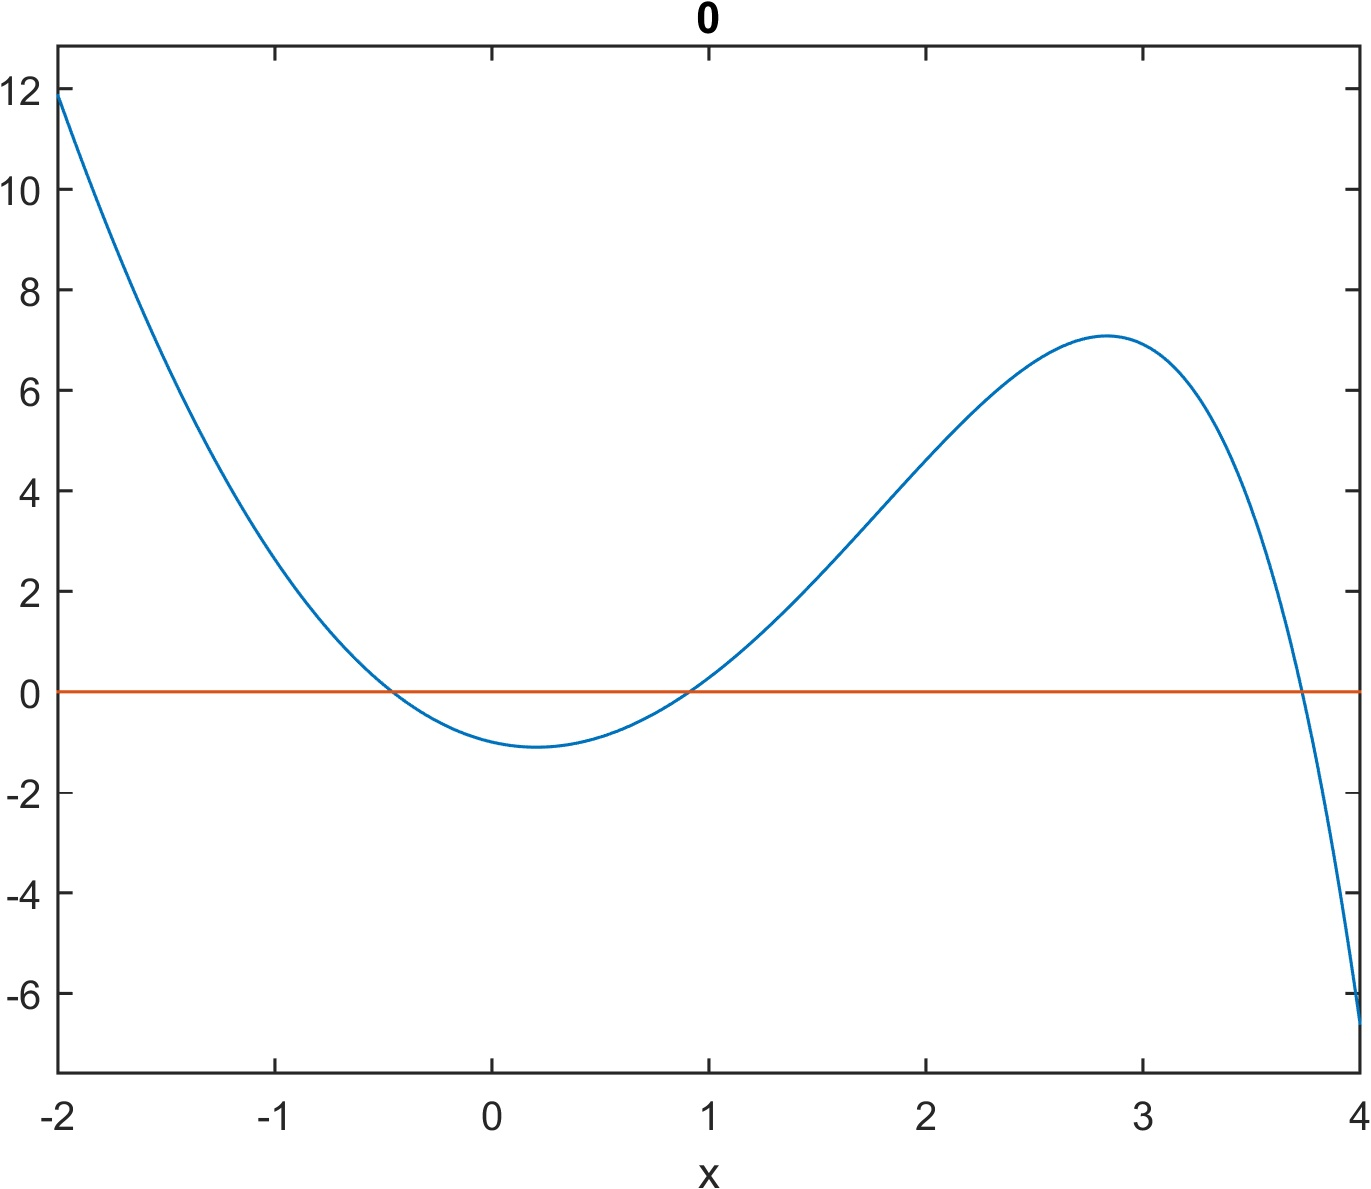
\includegraphics[height=7.5 cm]{estimate.jpg}
\\Fig.6.b For estimate
\end{center}

\begin{center}
\begin{tabular}{ |l| }
\hline
-1.000000000000000\\
 -0.586656659702033\\
  -0.469801907724523\\
  -0.459053916955023\\
  -0.458962274194841\\
  -0.458962274194841\\
  \hline
\end{tabular}
\end{center}
\begin{center}
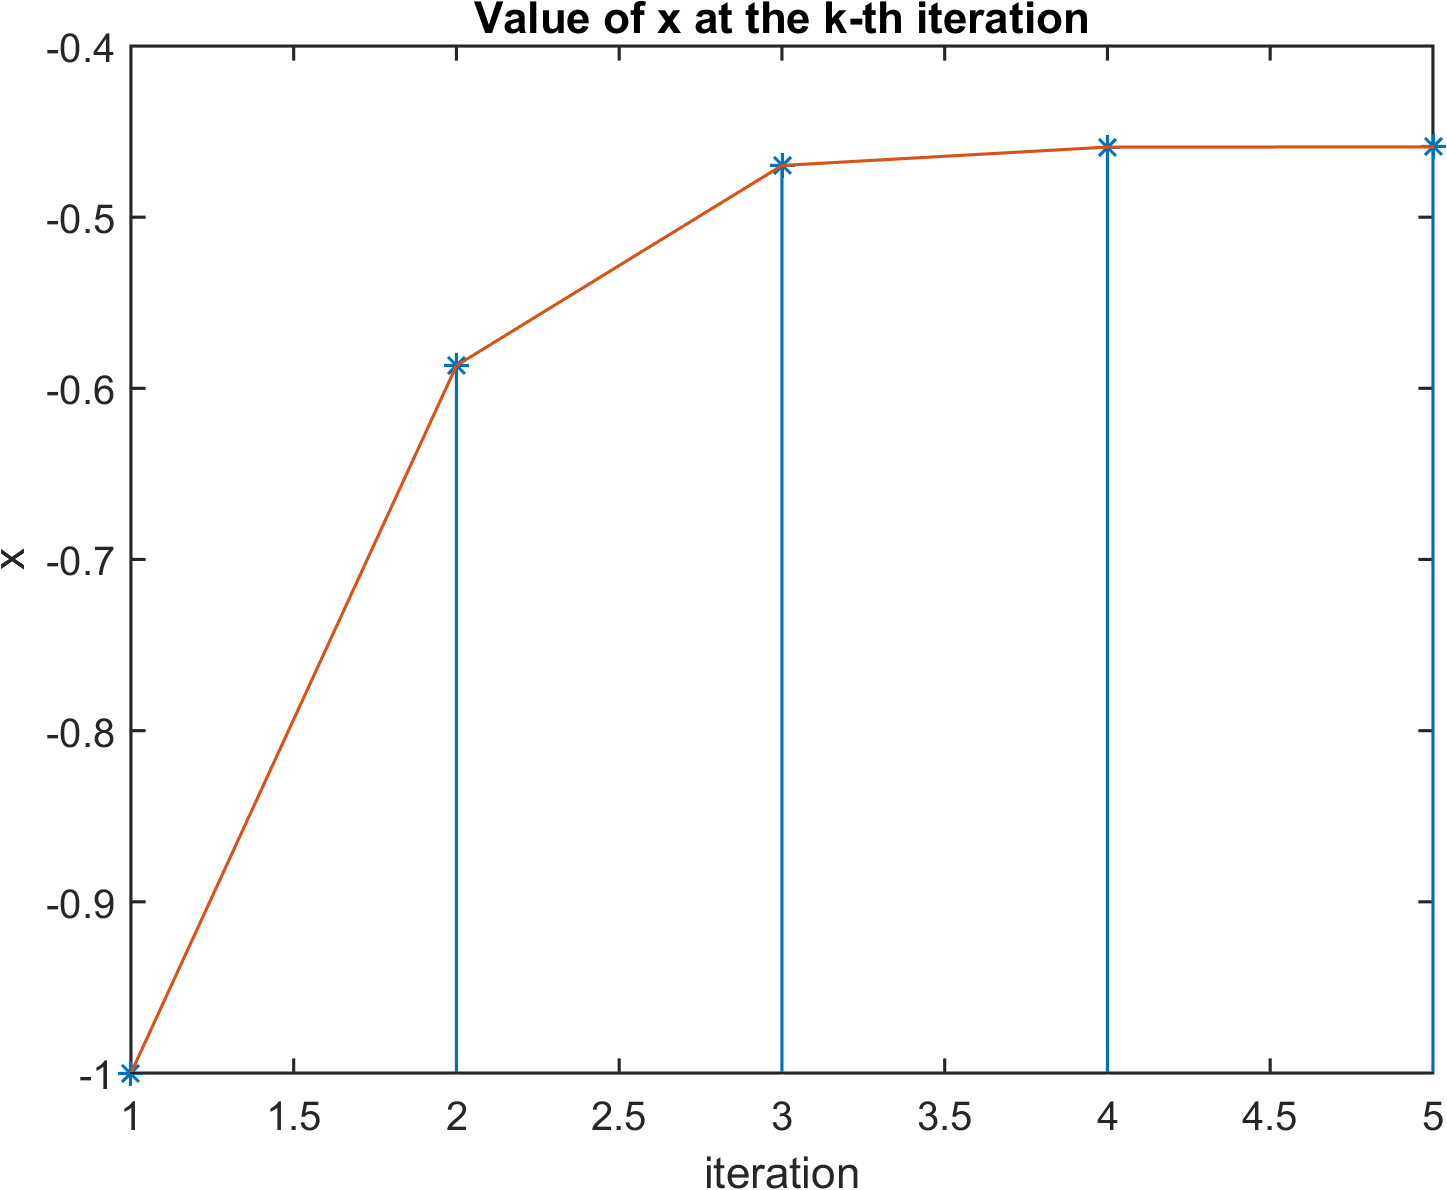
\includegraphics[height=7.5 cm]{fig6(2).png} \\
Fig.6.b.1 x in every iteration of Fix-Point method.
\end{center}

\begin{center}
\begin{tabular}{|l|}
 \hline
  1.000000000000000\\   0.914155281832543\\
   0.910017665783406\\

\hline
\end{tabular}
\end{center}
\begin{center}
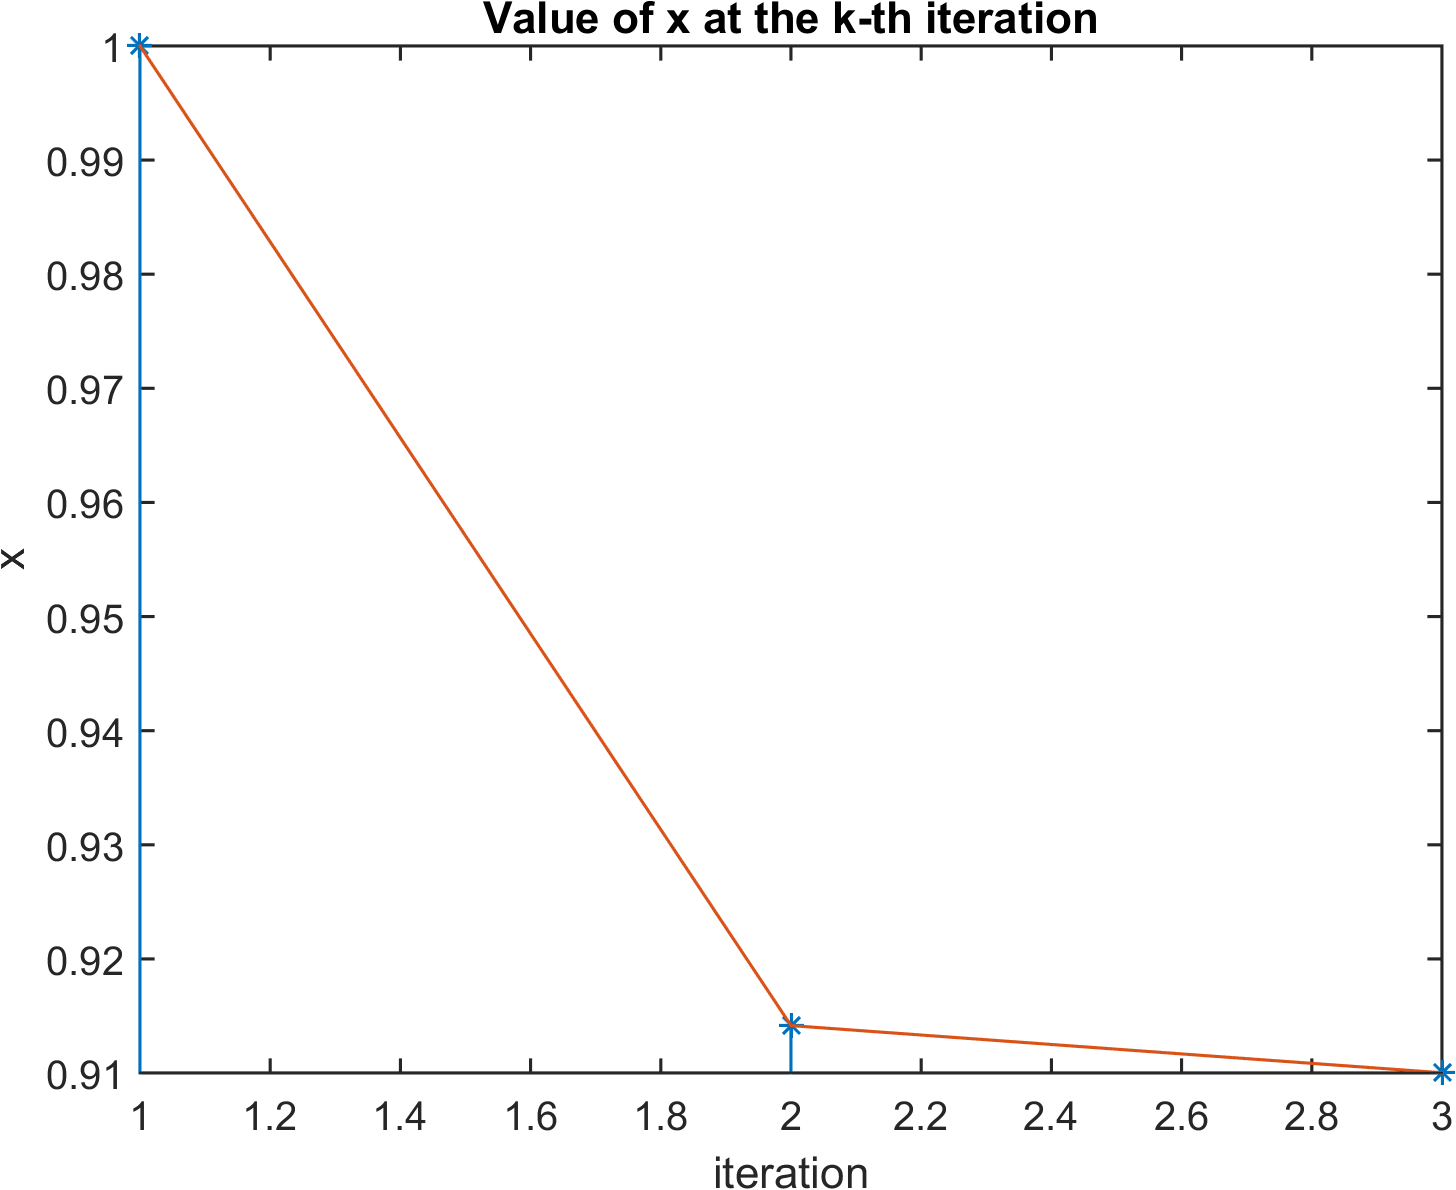
\includegraphics[height=7.5 cm]{fig6(4).png} \\
Fig.6.b.2 x in every iteration of Fix-Point method
\end{center}

\begin{center}
\begin{tabular}{ |l| }
\hline
 3.000000000000000\\   6.315435464093259\\
   5.474149482730207\\
   4.751646063932222\\
   4.201134675674261\\
   3.868723025906899\\
   3.747916887626595\\
   3.733278953493994\\
   3.733079065494898\\

\hline

\end{tabular}
\qquad
\begin{tabular}{ |l| }
\hline
4\\
 3.000000000000000\\   6.315435464093259\\
    4.000000000000000\\   3.784361145167370\\
   3.735379375079544\\
   3.733083897874097\\

\hline

\end{tabular}
\end{center}
What is shown below is the x of each iteration, using different initial point, 3 and 4 correspondingly. We find that Fix-Point method(Newton method here) is sensitive to initial value. A good initial estimate means very fast convergency.
\begin{center}
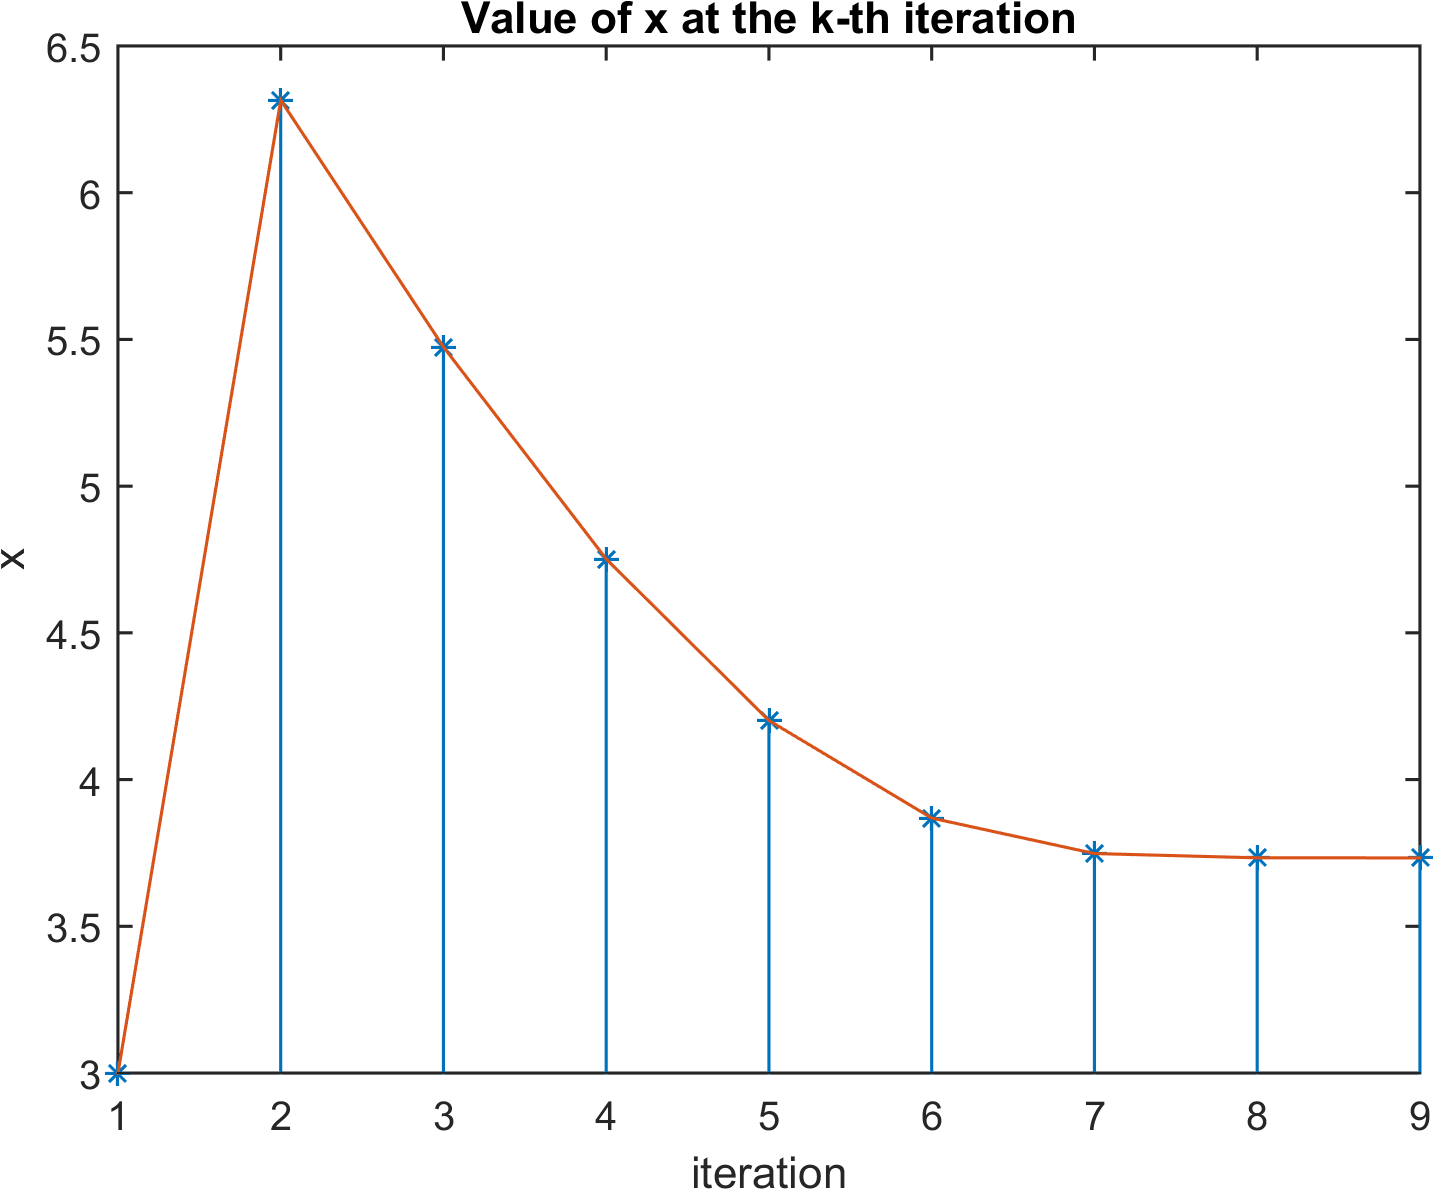
\includegraphics[height=5.5 cm]{fig6(5).png}
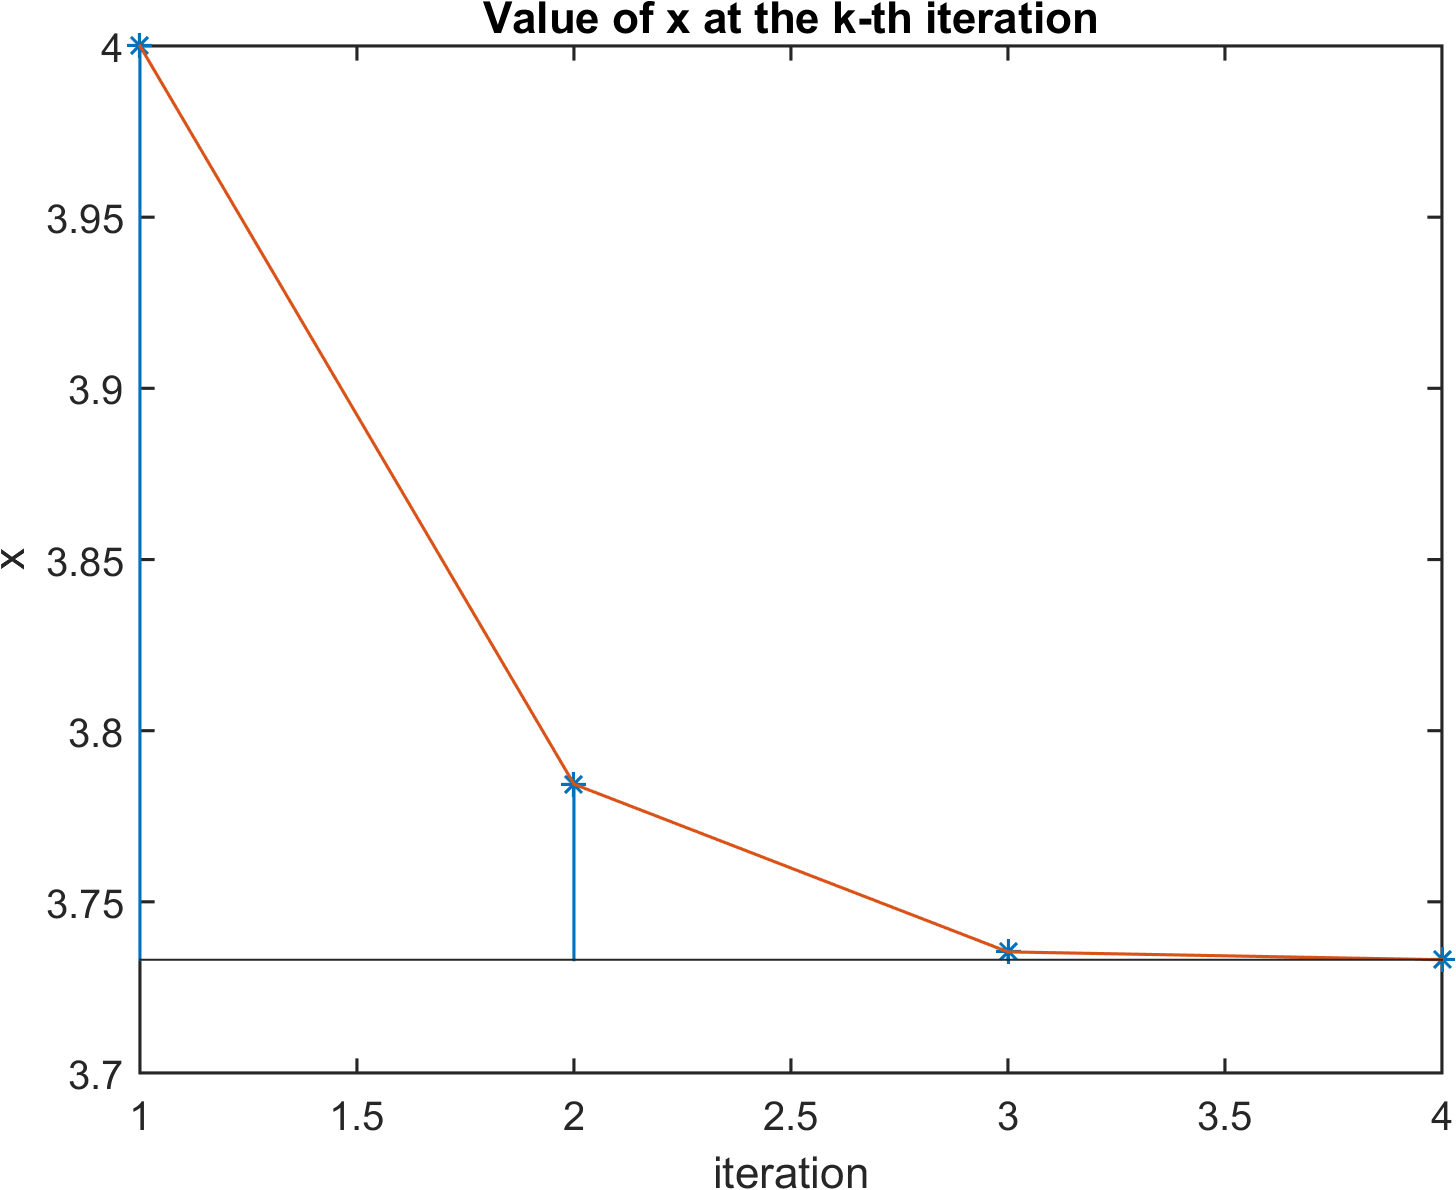
\includegraphics[height=5.5 cm]{fig6(6).png}
\\x in every iteration of Fix-Point method using different initial value of x.
\end{center}

Usage of Fix-Point method and the process to solve the problem is shown below:
\begin{lstlisting}
func3=@(x) 2*sin(pi*x)+x; %for problem a
func4=@(x) 3*x^2-exp(x); %for problem b
%% for estimate:
 figure('color',[1,1,1]);
 ezplot('x',[-2,2]);hold on;
 ezplot('2*sin(pi*x)',[-2,2]);
 figure('color',[1,1,1]);
 ezplot(func4,[-2,4]);hold on;
 ezplot('0',[-2,4]);

res4=FixPoint(func3,1); %TOL=10^-2, MaxIter=1000 is default, by using nargin.
res5=FixPoint(func4,-1);
res6=FixPoint(func4,0);
res7=FixPoint(func4,1);
res8=FixPoint(func4,3);
res9=FixPoint(func4,4);

\end{lstlisting}
\quad  The implement of Fix-Point method is shown below:
\lstinputlisting{FixPoint.m}

\section{Problem 7:}
{\bf{\emph{PROBLEM:}}}
 $g\in {{C}^{1}}[a,b]$ and p be in $(a, b)$ with $g(p) = p$ and $|g'(p)|>1$. Show that there exists a $\delta >0$ such that if $0<|{{p}_{0}}-p|<\delta $, then $|{{p}_{0}}-p|<|{{p}_{1}}-p|$. Thus, no matter how close the initial approximation ${{p}_{0}}$ is to $p$, the next iterate ${{p}_{1}}$ is farther away, so the fixed-point iteration does not converge if ${{p}_{0}}\ne p$.
\\ {\bf{\emph{SOLUTION:}}}
since $g\in {{C}^{1}}[a,b]$, which means derivation of g is continuous and $|g'(p)|>1$, which means it is bounded.Then we get:

 \[\exists \delta >0,\forall x\in [p-\delta ,p+\delta ]: \qquad |g'(x)|>1\]

 Here we can get a $\delta $, then we prove $\delta $ is what the we quests for. According to the Differential Mean Value Theorem��

\[\exists \xi \in [\min ({{p}_{0}},p),\max ({{p}_{0}},p)]:\qquad {{p}_{1}}-p=g({{p}_{1}})-g(p)=g'(\xi )({{p}_{0}}-p)\]

 As we know, $0<|{{p}_{0}}-p|<\delta \Rightarrow \xi \in [p-\delta ,p+\delta ]\Rightarrow |g'(\xi )|>1$, then we prove that

	\[ \left| {{p}_{1}}-p \right|=\left| g({{p}_{1}})-g(p) \right|=\left| {g}'(\xi )({{p}_{0}}-p) \right|>\left| {{p}_{0}}-p \right|\]

No matter how close to $p$ $p_0$ is, it can never turn back, thus the fixed-point iteration does not converge if ${{p}_{0}}\ne p$.

\end{document}




